\documentclass[a4paper,10pt]{article}
\usepackage[left=2cm, right=2cm, top=2cm, bottom=2cm]{geometry}
\usepackage{titlesec, enumitem, hyperref, xcolor, fontawesome5, tabularx, ltablex, tikz, graphicx, tcolorbox, parskip}

% TikZ Libraries
\usetikzlibrary{mindmap,shadows,shadings}

% Define colors
\definecolor{headerColor}{RGB}{0, 102, 102}
\definecolor{sectionColor}{RGB}{0, 102, 102}
\definecolor{borderColor}{RGB}{128, 128, 128}

% Define Section Style
\titleformat{\section}
{\huge\bfseries\color{sectionColor}} % Teal-colored, bold, larger text
{} % No numbering
{0pt} % No spacing
{} % No title prefix
[\vspace{0.2cm} \titlerule] % Adds spacing & horizontal line below

% Contact Information Layout
\begin{document}
	\begin{center}
		{\LARGE\textbf{\href{https://henribranken.github.io/MyCV/}{\faHandPointer~Henri Branken}}} \\[0.5cm]
		
		\begin{tabularx}{0.7\textwidth}{c X}
			\faHome & Potchefstroom (2531) \\
			\faEnvelope & \href{mailto:henri.branken777@gmail.com}{\textbf{henri.branken777@gmail.com}} \\
			\faPhone & \textbf{+27 (0) 82 785 5983} \\
			\faGithub & \href{https://github.com/HenriBranken}{\textbf{GitHub}} \\
			\faLinkedin & \href{https://www.linkedin.com/in/henri-branken-1423a2153/}{\textbf{LinkedIn}}
		\end{tabularx}
	\end{center}
	
	% Profile Image Styling
	\begin{minipage}{0.3\textwidth}
		\begin{tikzpicture}
			% Add a subtle shadow
			\shade[ball color=black!30, opacity=0.4] (0.2,-0.2) circle (2.2cm);
			
			% Clip and frame the image
			\clip (0,0) circle (2.2cm);
			\node[anchor=center] at (0,0) {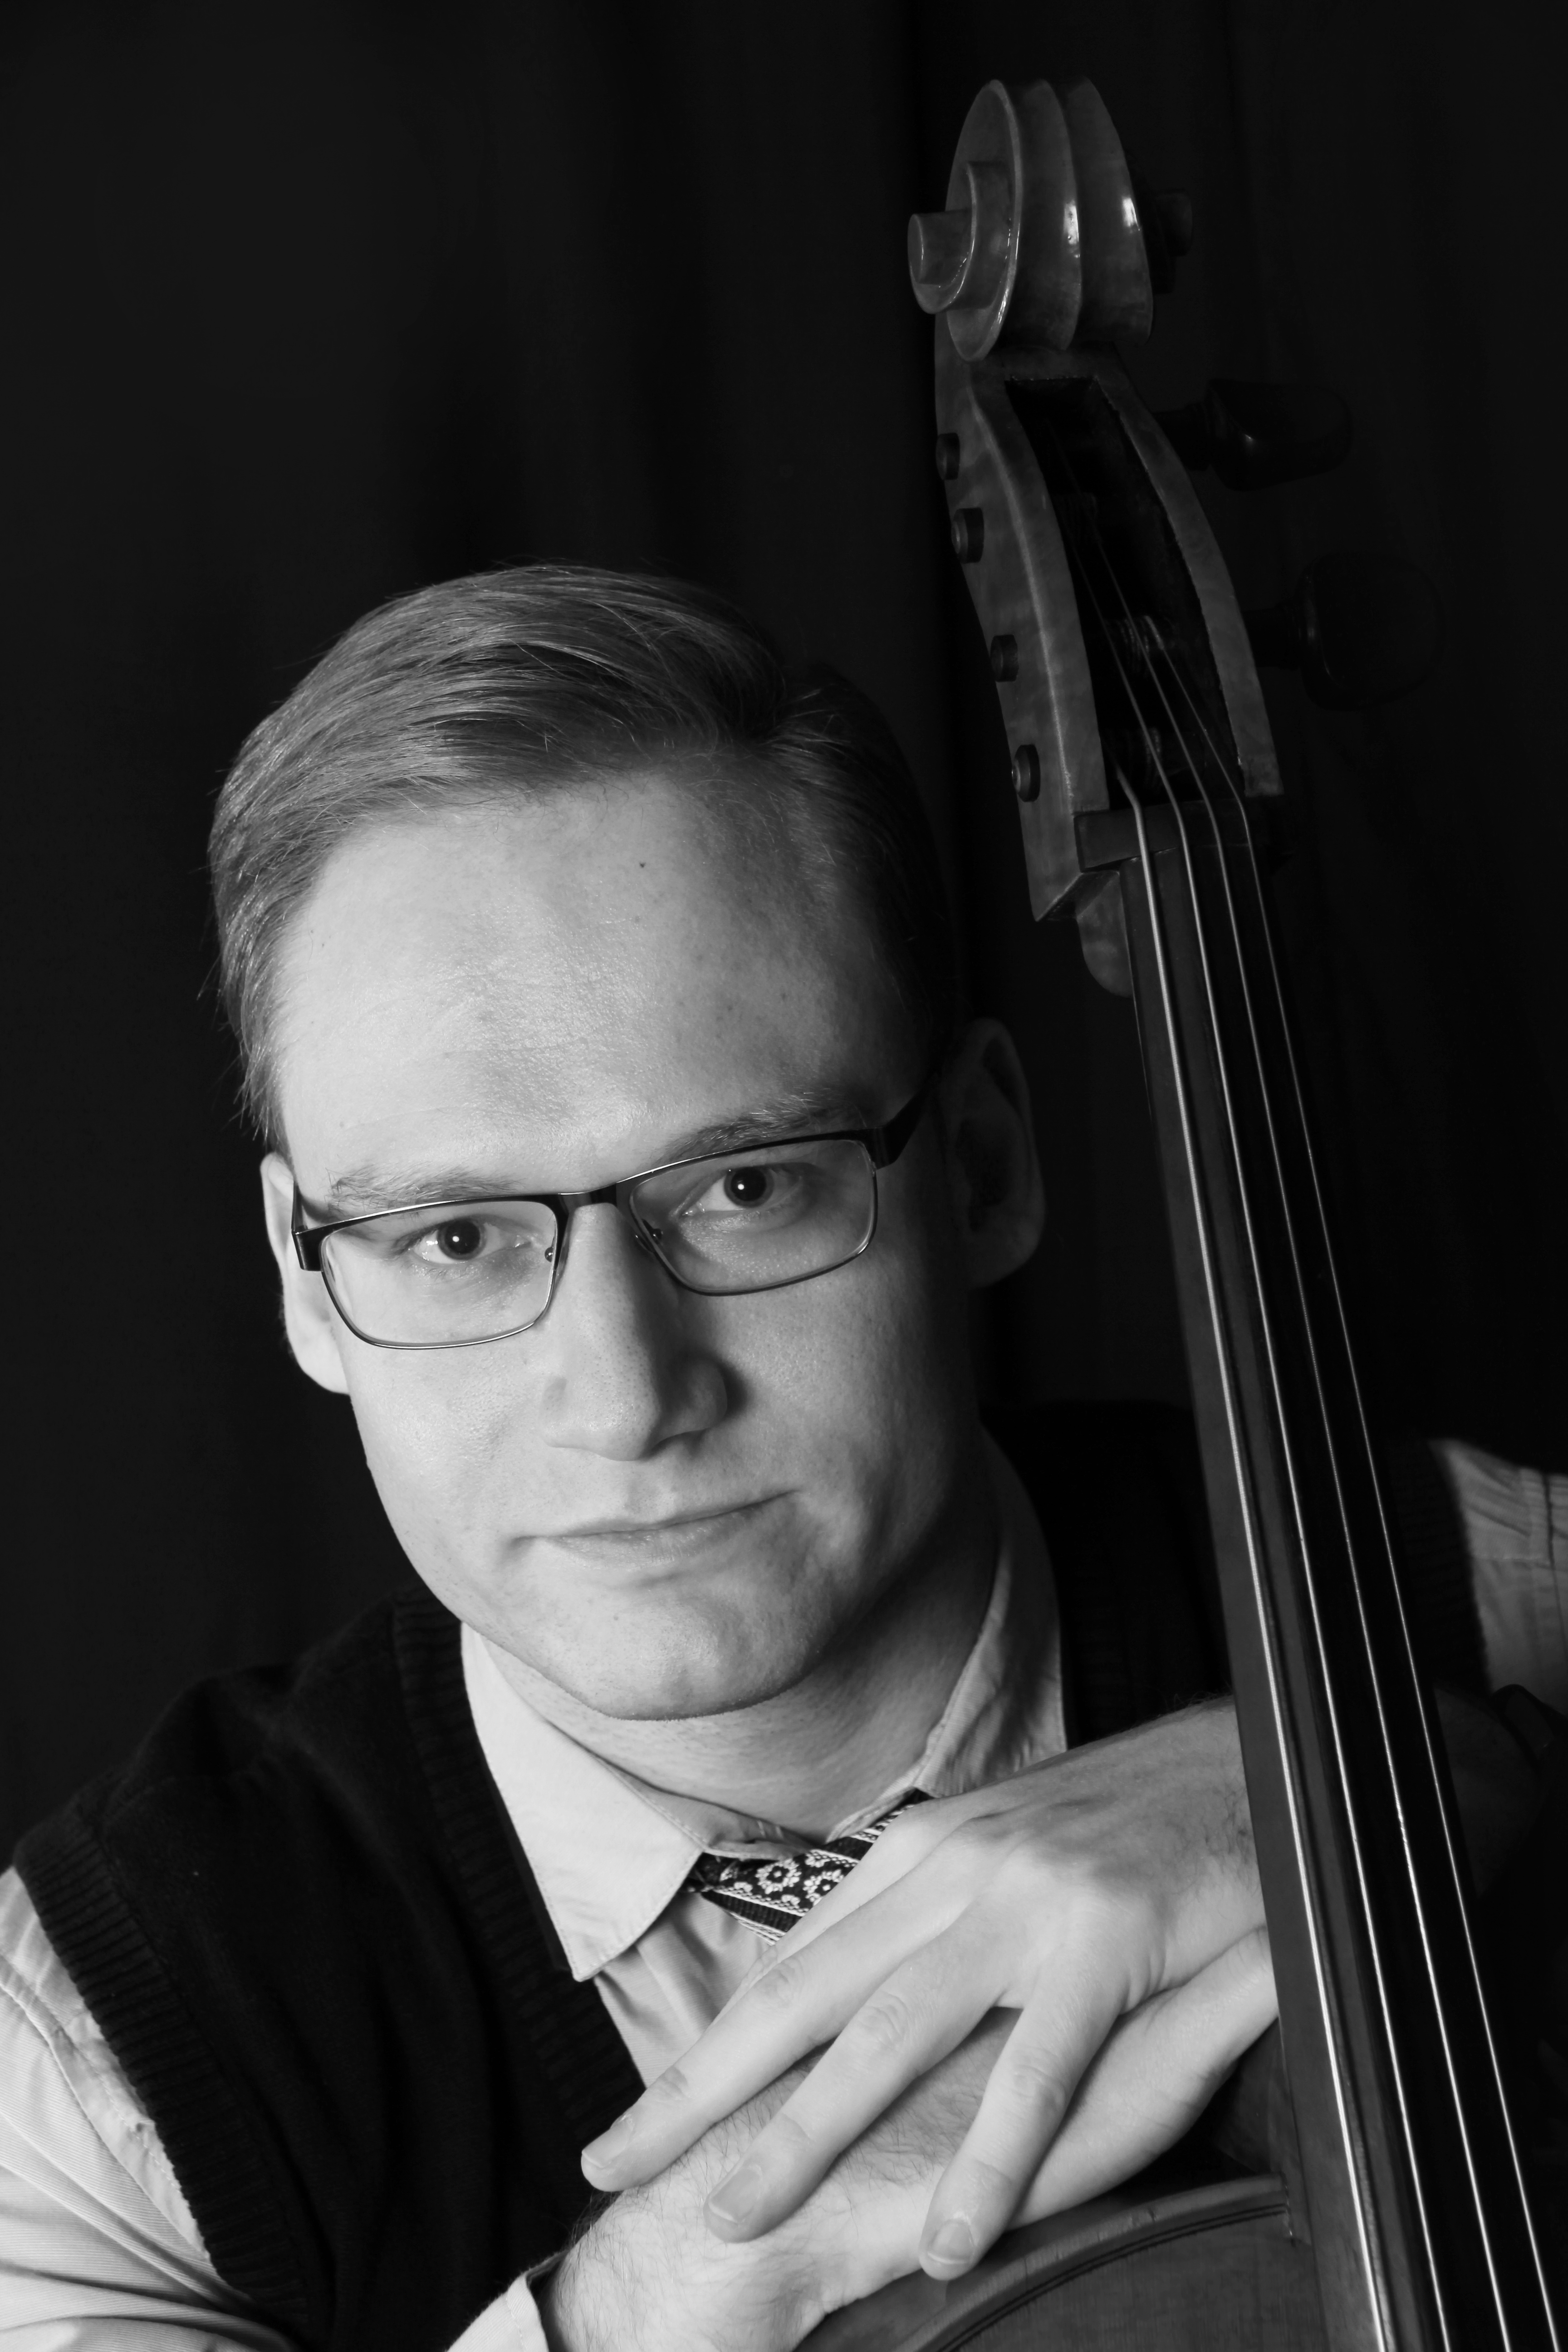
\includegraphics[width=4.4cm]{cello_11a}};
			
			% Add a decorative border
			\draw[thick, color=borderColor, dashed] (0,0) circle (2.2cm);
		\end{tikzpicture}
	\end{minipage}
	
	% Overview Section
	\section*{Overview}
	I hold a Master's Degree in Space Physics (Cum Laude) and have 3.5 years of experience as a Data Scientist at Matogen Applied Insights. I developed solutions such as a Portfolio Performance Monitor, a Credit Loss Model for a telecommunications company, and a PowerBI dashboard for monitoring agricultural nutrient distributions.
	
	To broaden my skill set, I completed a HyperionDev Bootcamp, mastering HTML, CSS, JavaScript, the MERN stack, and Java. This expanded my expertise in full-stack web development and database management. I later served as a Coding Mentor (July 2024 - January 2025).
	
	\section*{Languages}
	\begin{itemize}
		\item Afrikaans: Mother Tongue
		\item English: Fluent, Level 5 TEFL Certification
	\end{itemize}
	
	% Education and Training
	\section*{Education and Training}
	\renewcommand{\arraystretch}{1.1}
	\begin{tabularx}{\textwidth}{r l X}
		\textbf{2024/07--2025/03} & \multicolumn{2}{| l}{\textbf{HyperionDev} Code Reviewer \& Mentor} \\
		& \multicolumn{1}{| l}{\textbullet} & Evaluated coding submissions, provided feedback, and conducted live sessions. \\
		& \multicolumn{1}{| l}{\textbullet} & Refactored \href{https://github.com/HenriBranken/AcademicPortfolio/blob/main/06-010-1\_React\%20\textendash\%20Testing\%20a\%20React\%20App.pdf}{\textbf{task contents}} for course syllabi. \\
		& \multicolumn{1}{| l}{\textbullet} & Conducted \href{https://github.com/HenriBranken/AcademicPortfolio/blob/main/Academic\%20Onboarding\%20Session.pdf}{\textbf{onboarding sessions}} for new students. \\
		
		\textbf{2023/01--2023/09} & \multicolumn{2}{| l}{\textbf{HyperionDev Full Stack Web Dev Bootcamp}} \\
		& \multicolumn{1}{| l}{\textbullet} & Completed coursework in MERN stack, Java, and database management. \\
		& \multicolumn{1}{| l}{\textbullet} & Awarded \href{https://www.facebook.com/henri.branken.9/posts/pfbid02gUh1H3ovPTfn4TLrr3ZYFWzhcEyuDte2xsZTLbPjHiNZStTRPEArNnius6T5Bj5rl}{\textbf{Student of the Month}}. \\
		
	\end{tabularx}
	
	% Skills Mindmap
	\begin{center}
		\tikz[mindmap, text=white, grow cyclic,
		root concept/.style={concept color=red!20, font=\Huge\bfseries},
		level 1 concept/.append style={
			sibling angle=100, % More spacing between categories
			level distance=6.5cm,
			every child/.style={concept color=blue!20, font=\large\bfseries}
		},
		level 2 concept/.append style={
			sibling angle=50,
			level distance=3.5cm,
			every child/.style={concept color=red!20, text=black}
		}]
		\node [concept, concept color=black] {Henri's Skills}
		child {node [concept] {Full-Stack \\ Web Dev}
			child {node [concept] {PHP}}
			child {node [concept] {Java}}
			child {node [concept] {MERN}}
			child {node [concept] {HTML, CSS, \\ JavaScript}}
		}
		child {node [concept] {Data Science}
			child {node [concept] {EDA, Wrangling}}
			child {node [concept] {PowerBI, Tableau}}
			child {node [concept] {Git CLI, GitHub}}
			child {node [concept] {SQL, PySpark}}
			child {node [concept] {Python, \\ Jupyter Notebook}}
		}
		child {node [concept] {Research}
			child {node [concept] {\LaTeX}}
			child {node [concept] {TiKZ}}
			child {node [concept] {Maths, Physics}}
			child {node [concept] {LibreOffice Suite}}
			child {node [concept] {ChatGPT}}
		}
		child {node [concept] {Teaching}
			child {node [concept] {TEFL Diploma}}
			child {node [concept] {Coding Mentor}}
			child {node [concept] {Code Reviewer}}
		};
	\end{center}
	
	% References Section
	\section*{References}
	\begin{tabularx}{\textwidth}{l X}
		\textbf{Seraaj De Villiers} & HyperionDev \\
		& \faEnvelope \quad \href{mailto:seraajd@hyperiondev.com}{seraajd@hyperiondev.com} \\[0.2cm]
		
		\textbf{Prof. Christo Venter} & North-West University \\
		& \faEnvelope \quad \href{mailto:christo.venter@nwu.ac.za}{christo.venter@nwu.ac.za} \\[0.2cm]
		
		\textbf{Mr. Jacobus Eksteen} & CEO, Matogen Applied Insights \\
		& \faEnvelope \quad \href{mailto:jacobus.eksteen@ai.matogen.com}{jacobus.eksteen@ai.matogen.com} \\
	\end{tabularx}
	
\end{document}
